\chapter{Overview of CryptDB}
\label{chp:overview_cryptDB}

\section{System Architecture}

CrytpDB's architecture is divided into two pieces. The proxy server and the database server.

The proxy server is an intermediate server placed between the application server (used by the application to manage key setup and interacting with clients) and the database server. Its purpose is to intercept queries going from the application to the database and anonymize the information of the query so possible eavesdropping attackers are not able obtain any sensible information. %Kommentere at Microsoft hevder å ha brukt freq attack her.
Another vital part of the proxy server's domain is to issue queries to the database that adjusts the encryption layer (or onion layer) of the column(s) that the user has issued a query on, which will be discussed in section \ref{adjust_enc_level}

\begin{figure}[h]
	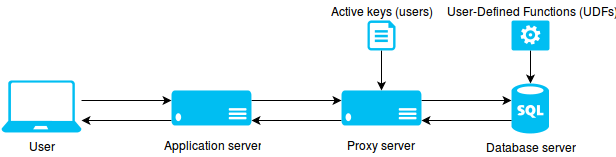
\includegraphics[scale=0.6]{CryptDB_Plain.png}
	\caption{System architecture of CryptDB interacting with a client application}
	\label{cryptdb_plain}
\end{figure}


Explain the client application\\
Explain the use of the proxy server\\
Explain the key storage\\
Explain the use of the database server\\

\section{SQL-Aware Encryption and the Onion Scheme}

CryptDB uses an encryption scheme called \emph{SQL-aware encryption} or \textit{onion encryption}. Basically, this means that the encryption scheme is a collection of different schemes, each providing different levels of security and computations to be executed. Data items stored using CryptDB are encrypted multiple times using these different schemes, or layers, of encryption.

Må skrive en del mer på introen her.\\

\Gls{random_onion} is the highest security level in CryptDB and provides the maximum security found in encryption scheme. It uses a strong block cipher such as Blowfish or \Gls{aes} in \Gls{cbc_mode} mode and a random initialization vector (IV) to ensure that the block cipher is probabilistic. \Gls{random_onion}, being the maximum security level provided, does not allow any computation to be done on the encrypted data. In other terms, this level is a natural choice for sensitive data that are only meant to be read. When a block cipher is probabilistic, it has properties such that when encrypting the same message $m_1$ multiple times, the resulting ciphertexts are unequal. For example, given two encryptions of the same plaintext $c_1 = E_k(m_1)$ and $c_2 = E_k(m_1)$, the resulting ciphertexts are $c_1$ and $c_2$ such that $c_1 \neq c_2$.



Where \Gls{random_onion} allows no computation to be done on the encrypted data, the next layer does. \Gls{deterministic_onion} is an encryption scheme enabling the application to perform standard SQL operations such as equality checks, distinct, group by and count. By allowing these sorts of computation, the application leaks information to an adversary. In particular, it leaks which ciphertexts that decrypts to the same plaintext value. Following the previous example; if the scheme encrypted the message $M_1$ two times, the resulting ciphertexts $C_1$ and $C_2$ are equal. \Gls{deterministic_onion} is a deterministic scheme which, to be used correctly, should be a \Gls{prp}. In order to cope with leaking prefix equality, the authors have designed their own version of the CMC mode \cite{CryptDB_Main_Paper}.



Since \Gls{sql} also allows the user to compute on order relations between items, CryptDB introduces an \Gls{ope_onion} scheme. \citep{CryptDB_Main_Paper} This scheme takes starting point in a requirement where the sort order of the ciphertext matches the sort-order of the corresponding decrypted plaintexts. It also requires that the scheme reveals no other information about the plaintexts, other than the respective order. This common operation in \Gls{sql} supports order comparison, which can be used for range checks, ranking, sorting, and extracting minimum and maximum values. Popa et al. \cite{CryptDB_OPE_Encoding} introduces a scheme called \Gls{mOPE} where the main technique is mutable ciphertexts. Mutability (or malleability) is a cryptographic property allowing transformation of one ciphertext into another. More formally, given a plaintext $m_1$, it is possible to transform it into a valid encryption $f(m_1)$ by using a valid function $f$ without further knowledge of $m_1$.

\Gls{mOPE} uses a balanced binary tree for searching which contains encryptions of all the plaintext's values and a table of \Gls{ope_onion} encodings where the encoded value of a ciphertext is its path from the root to the particular node in the binary tree. If $y$ is greater than $x$, then $y$ will be located to the right of $x$ in the tree. It also uses an interactive protocol when inserting a value into the search tree, where the server and the client plays a query game. The client asks for the encrypted root node, decrypts it and determines whether the value to be inserted is smaller or larger than the root. It replies to the server with a $0$ or $1$, making the server traverse the tree to the left or right and replying with the next encrypted node. This little game continues until there are no child nodes. In order to avoid the tree being too deep, \Gls{mOPE} uses a tree-balancing transformation summary which describes operations (most of them split-and-merge operations) that are completely done by the server. This balancing procedure ensures that the height of the tree is bounded by $\log(N)$, where $N$ is the number of encrypted values. Because both client and server needs a shared understanding of the structure of the search tree, the client computes a Merkle hash of the root of the tree. A Merkle tree is a tree where every parent node is labelled with the hash of all of its children's labels.\cite{Merkle} By performing the Merkle hash, the client is able to check whether the server behaves malicious or not (Malicious in this setting would be if the server performed other operations than the client requested) by comparing its own Merkle hash of the root with the one delivered by the server.



Another vital part of \Gls{sql} is the ability to perform addition and multiplication. For CryptDB to be able to perform these operations, it utilizes a \Gls{hom_onion} scheme. As previously described, homomorphic encryption is a technique that enables computation on encrypted data without decrypting it first.

CryptDB uses Pailler multiplication, which in practice is the same as performing summation on two items. $HOM_k(x) * HOM_k(y) = HOM_k(x + y)$.


Join (Join and OPE-Join)


Word Search (SEARCH)


\section{Adjusting the Encryption Level Based on the Query}
\label{adjust_enc_level}

A story about a spies, a castle and some walls. Metaphor, bitches.


\subsection{Threats}

\subsection{Security}